\vspace*{4cm}
\part{Bluetooth Mesh}\label{part:BluetoothMesh}
Raffael Anklin
\vspace*{\fill}
\clearpage

\section{Einleitung und Grundlagen}\label{sec:EinleitungBluetooth}


Bluetooth Mesh ist ein auf dem Bluetooth-Standard aufbauendes Mesh-Netzwerk. Der Standard wurde im Jahr 2017 von der Bluetooth-SIG vorgestellt. Das Ziel des Standards ist es die Reichweite und das Einsatzgebiet von Bluetooth-Geräten zu erweitern. Somit sollen in Zukunft Lichtschalter und Lampen, sowie Sensoren und Aktoren im Heimbereich, Industriebereich und diversen Anwendungsbereichen mittels Bluetooth-Technologie verbunden werden.  \\

\begin{figure}[!htbp]
	\begin{minipage}{0.49\textwidth}
		\centering
		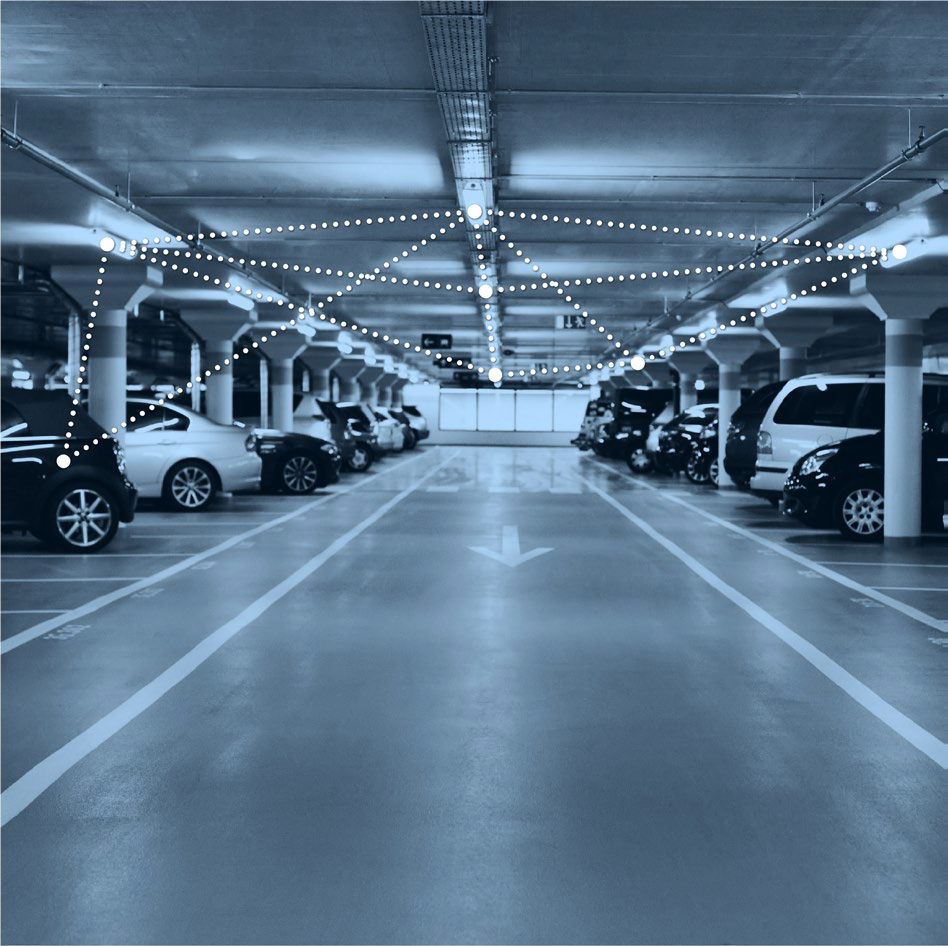
\includegraphics[width=\textwidth]{Bluetooth_Mesh_CarPark_Example.png}
		\caption[Parkhaus mit Bluetooth-Mesh]{Parkhaus mit Bluetooth-Mesh \cite{bluetooth_sig_mesh-technology-overviewpdf_2020}}
		\label{fig:BluetoothMeshParkingExample}
	\end{minipage}
	\begin{minipage}{0.49\textwidth}
		\centering
		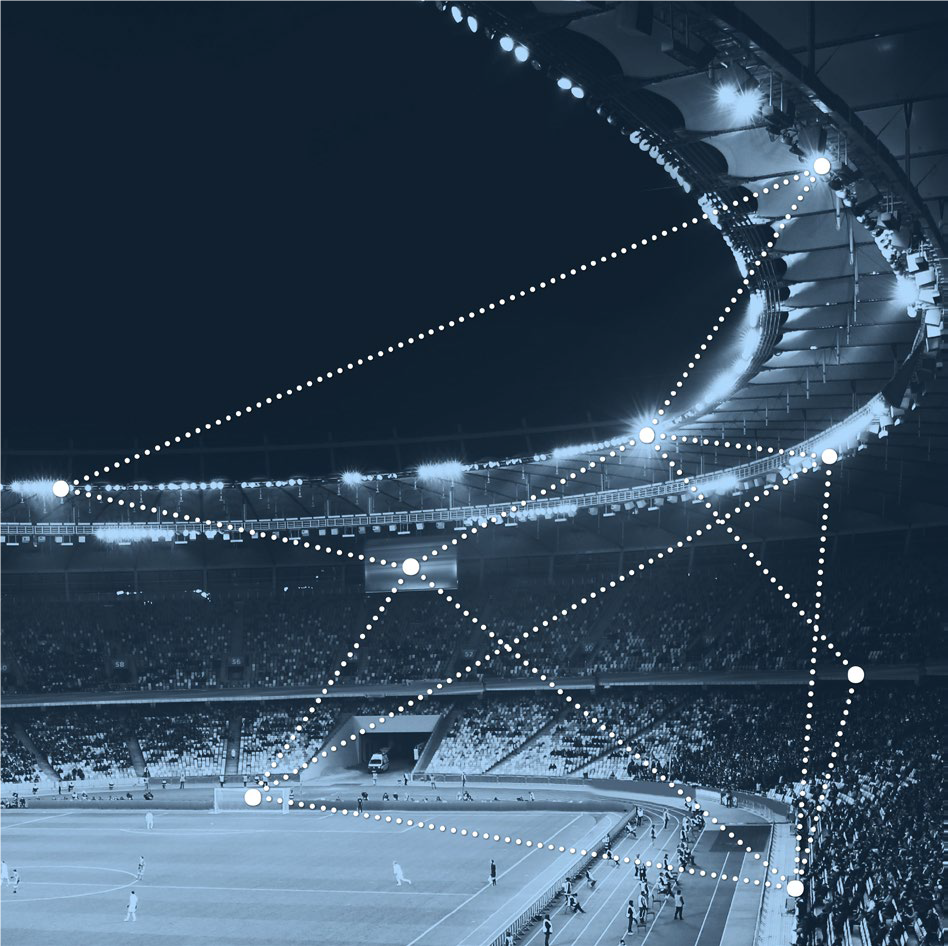
\includegraphics[width=\textwidth]{Bluetooth_Mesh_Stadium_Example.png}
		\caption[Stadion mit Bluetooth-Mesh]{Stadion mit Bluetooth-Mesh \cite{bluetooth_sig_mesh-technology-overviewpdf_2020}}
		\label{fig:BluetoothMeshStadiumExample}
	\end{minipage}
\end{figure}


Die Technologie baut auf den weit verbreitetem BLE-Standard auf, welcher in einer viel zahl von Endgeräten verbaut ist. Ab BLE-Version 4.0 könnten sich die Geräte zu einem Mesh-Netzwerk verbinden. Im Anschluss wird der Netzaufbau kurz erklärt und der Leser mit dem Funktionsprinzip des Mesh-Stacks vertraut gemacht. \\

\paragraph{Provisioning}

Das Einbinden neuer Teilnehmer in ein Bluetooth-Mesh Netzwerk findet über den Provisioning-Prozess statt. Die Rolle des Provisioners kann ein Smartphone, Laptop oder ein berechtigter Mesh-Teilnehmer übernehmen. Ähnlich wie beim anmelden bei einem WLAN-Netzwerk teilt der Provisioner dem neuen Teilnehmer die Zugangsdaten (Netzwerkschlüssel, etc.) mit. Abschliessend beginnt das neue Gerät im Netzwerk als Node zu operieren. \\

\paragraph{Managed-Flooding}

Bluetooth-Mesh basiert auf dem Managed-Flooding Prinzip. Einfach erklärt wiederholen alle Nodes, abhängig von verschiedenen Bedingungen, jede empfangende Nachricht (Relaying). Somit gelangen die Daten über Zwischenstationen (Hops) zum Ziel. Nachrichten welche bereits  wiederholt wurden werden nicht erneut gesendet. Zusätzlich wird ein Time-To-Live Zähler zu jeder Nachricht mitgegeben. Dieser gibt an, wie oft die Mitteilung erneut gesendet wird. \\

\paragraph{Models}

Um die Funktion von Nodes (Lichtschalter, Lampe, Temperatursensor, etc.) zu unterscheiden, werden sogenannte Models definiert. Jedes Model spezifiziert Zustände (Licht EIN / Licht AUS), welche als States bezeichnet werden. Weiterhin sind Models in drei Kategorien eingeteilt: Server-, Client- und Control-Models. Diese Einteilung schreibt vor, ob die Zustände des Nodes zur Veränderung Angeboten werden (Server-Model z.B. Lampe), Zustände verändert werden (Client-Model z.B. Schalter) oder beides möglich ist (Control-Model z.B. Pumpe). Mithilfe dieser Normen lassen sich Geräte von unterschiedlichen Hersteller vereinen, sofern keine Hersteller spezifischen Models verwendet wurden. 

\begin{figure} [H]
	\centering
	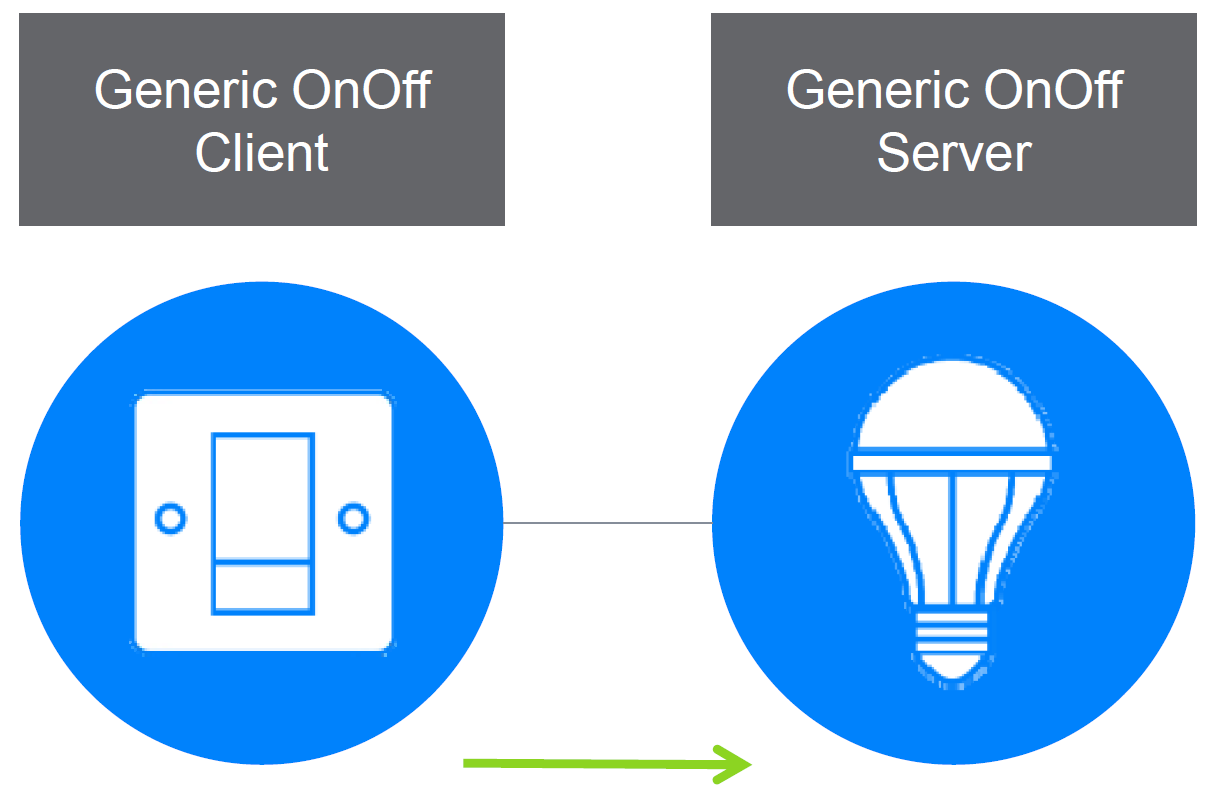
\includegraphics[width=0.6\textwidth]{Bluetooth_Mesh_Client_Server_Prinzip.PNG}
	\caption{Client - Server Prinzip Bluetooth Mesh \cite{bluetooth_sig_mesh-technology-overviewpdf_2020}} 
	\label{fig:BTMeshClientServerPrinzip}
\end{figure}

\paragraph{Adressierung}

Zur Identifizierung im Netzwerk besitzt jeder Node eine Unicast-Address (einzigartige Adresse). Um mehrere Nodes zu einer Gruppe zusammenzufassen, werden Group-Addresses vergeben. Die Beziehungen zwischen Nodes werden durch Publishen (Veröffentlichen) oder Subscriben (Abonnieren) auf Adressen geregelt. Im Anwendungsfall Publisht der Client (Schalter) an die Adresse auf welche einer oder mehrere Server (Lampe/Lampen) Subscriben. Wie in Abbildung \ref{fig:BTMeshPublishSubscribePrinzip} ist das Unterscheiden von Bereichen mittels Gruppen möglich. Ein Node kann gleichzeitig an mehrere Adressen Publishen und Subscriben, was zu beliebig komplexen Aufbauten führt. 


\begin{figure} [H]
	\centering
	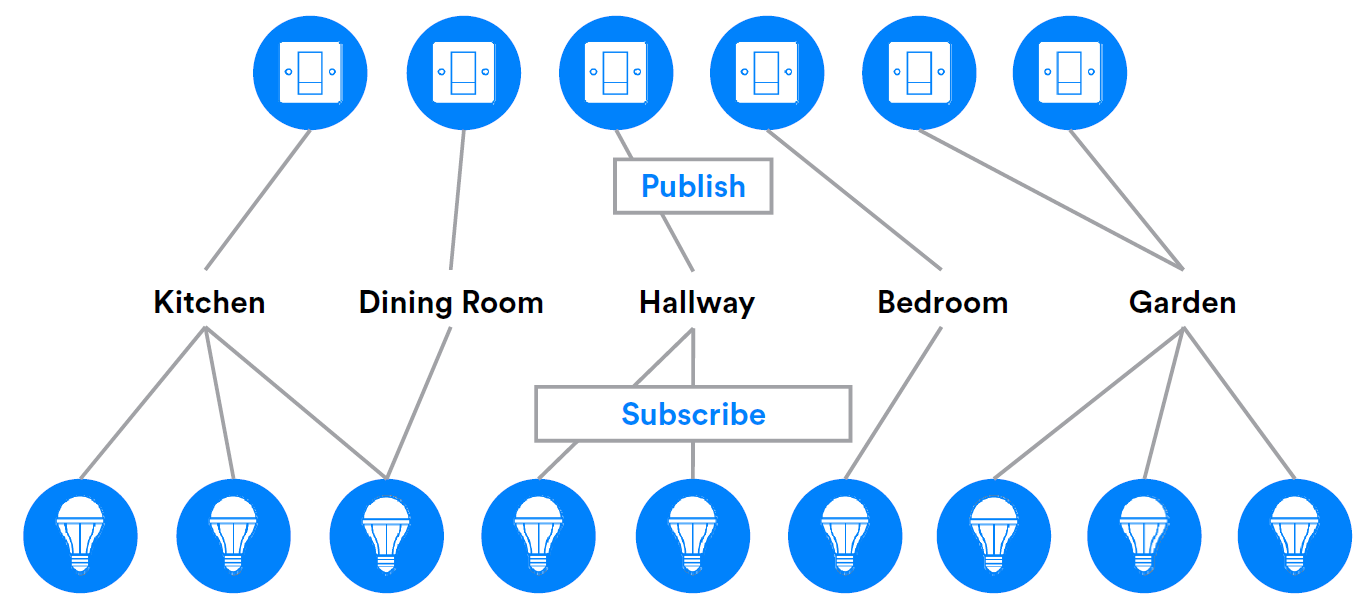
\includegraphics[width=1.0\textwidth]{Bluetooth_Mesh_Publish_Subscribe_Prinzip.PNG}
	\caption{Publish - Subscribe Prinzip Bluetooth Mesh \cite{bluetooth_sig_mesh-technology-overviewpdf_2020}} 
	\label{fig:BTMeshPublishSubscribePrinzip}
\end{figure}








